\documentclass[aspectratio=169,10pt]{beamer}

\usepackage[utf8]{inputenc}
\usepackage[T1]{fontenc}
\usepackage[english]{babel}
\usepackage{lmodern}
\usepackage{graphicx}
\usepackage{tikz}
\usepackage{booktabs}
\usepackage{amsmath, amssymb}
\usepackage{xcolor}
\usepackage{hyperref}
\usepackage{caption}

\usetikzlibrary{arrows.meta, positioning, shapes.geometric, fit, backgrounds, calc}

% --- Theme: clean medical palette ----------------------------------------
\usetheme{Madrid}
\usecolortheme{whale}

\definecolor{medBlue}{RGB}{0,73,114}
\definecolor{medTeal}{RGB}{0,128,128}
\definecolor{medAccent}{RGB}{200,80,40}
\definecolor{medSoft}{RGB}{235,242,247}

\setbeamercolor{structure}{fg=medBlue}
\setbeamercolor{title}{fg=white,bg=medBlue}
\setbeamercolor{frametitle}{fg=white,bg=medBlue}
\setbeamercolor{block title}{bg=medTeal,fg=white}
\setbeamercolor{block body}{bg=medSoft,fg=black}
\setbeamercolor{alerted text}{fg=medAccent}

\setbeamertemplate{navigation symbols}{}
\setbeamertemplate{footline}[frame number]
\setbeamerfont{title}{size=\Large,series=\bfseries}
\setbeamerfont{frametitle}{size=\large,series=\bfseries}

% --- Metadata ------------------------------------------------------------
\title[Geometric humeral analysis]{Interpretable Geometric Analysis of the Humerus\\ in Fat-Suppressed Shoulder MRI}
\subtitle{Toward localization of rotator cuff tears via foundation-model segmentation\\ and direction-aware geometric features}
\author[UNAL]{Marco Paluszny Kluczynsky \and Gustavo Adolfo P\'erez\\\small Universidad Nacional de Colombia}
\institute[UNAL]{Topics in Computational Geometry --- UNAL, Colombia}
\date{1\textsuperscript{st} UEMS Congress 2026 \\ Leuven, Belgium --- 27--30 May 2026}

\begin{document}

% Slide 1 -- Title
\begin{frame}[plain]
  \titlepage
  \begin{center}
    \footnotesize \textcolor{medTeal}{Bridging computational geometry and musculoskeletal radiology}
  \end{center}
\end{frame}

% Slide 2 -- Clinical problem (text only)
\begin{frame}{The clinical problem: rotator cuff tears}
  \begin{block}{Why it matters}
    \begin{itemize}
      \item Rotator cuff disease affects \alert{$>$30\% of adults over 60}, the leading cause of shoulder pain and disability.
      \item Tears arise from acute trauma or chronic degeneration (microtrauma + tendon-insertion ischemia).
      \item Accurate \alert{localization} --- which tendon, where along the insertion --- drives surgical planning.
    \end{itemize}
  \end{block}
\end{frame}

% Slide 2b -- Glenohumeral schematic (image only)
\begin{frame}{Anatomy of the glenohumeral joint}
  \centering
  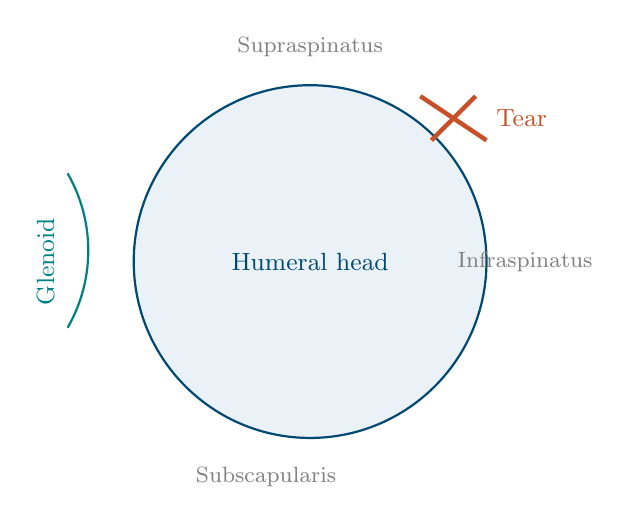
\begin{tikzpicture}[scale=1.4]
    \draw[thick, medBlue, fill=medSoft] (0,0) circle (1.6);
    \node[medBlue] at (0,0) {\small Humeral head};
    \draw[thick, medTeal] (-2.2,-0.6) arc (-30:30:1.4);
    \node[medTeal, rotate=90] at (-2.4,0) {\small Glenoid};
    \draw[medAccent, ultra thick] (1.1,1.1) -- (1.5,1.5);
    \draw[medAccent, ultra thick] (1.0,1.5) -- (1.6,1.1);
    \node[medAccent, right] at (1.6,1.3) {\small Tear};
    \node[gray, font=\footnotesize] at (0,1.95) {Supraspinatus};
    \node[gray, font=\footnotesize] at (1.95,0) {Infraspinatus};
    \node[gray, font=\footnotesize] at (-0.4,-1.95) {Subscapularis};
  \end{tikzpicture}
  \\[0.6em]
  {\footnotesize Axial schematic of the glenohumeral joint. Tears disrupt the articular contour focally.}
\end{frame}

% Slide 2c -- Diagnostic challenge (text only)
\begin{frame}{Why is this hard to read on MRI?}
  \begin{block}{Diagnostic challenge}
    \begin{itemize}
      \item MRI reading is \alert{expert-dependent} and time-consuming.
      \item Inter-vendor variability (SIEMENS / GE / Philips) complicates automation.
      \item Subtle partial tears can be missed on a single slice; 3D context is needed.
    \end{itemize}
  \end{block}

  \begin{block}{Equity-of-access gap}
    \begin{itemize}
      \item Limited access to subspecialty musculoskeletal radiology in low-resource settings.
      \item In Colombia, regions like \alert{Choc\'o} (Quibd\'o) lack dedicated MSK readers despite having modern MRI.
      \item Automated, interpretable tools can support generalist radiologists.
    \end{itemize}
  \end{block}
\end{frame}

% Slide 3 -- Imaging context
\begin{frame}{Imaging context: why fat-suppressed axial MRI?}
  \begin{columns}[T]
    \begin{column}{0.55\textwidth}
      \begin{block}{Fat saturation (fs)}
        \begin{itemize}
          \item Selective RF pulse \alert{nulls fat signal} $\Rightarrow$ subcutaneous and marrow fat appear dark.
          \item Cortical bone, tendon, edema and joint fluid become \alert{conspicuous}.
          \item Standard sequences here: \textbf{PD-fs} (anatomical detail + edema sensitivity) and \textbf{T1-fs}.
        \end{itemize}
      \end{block}

      \begin{block}{Why the axial plane?}
        \begin{itemize}
          \item The humeral head appears as \alert{nested circles} that grow to a maximum (the ``equator'') and shrink.
          \item Yields a clean \emph{area-vs-slice} curve we can validate geometrically.
          \item Direct view of the glenohumeral contact surface where most tears manifest.
        \end{itemize}
      \end{block}
    \end{column}
    \begin{column}{0.45\textwidth}
      \centering
      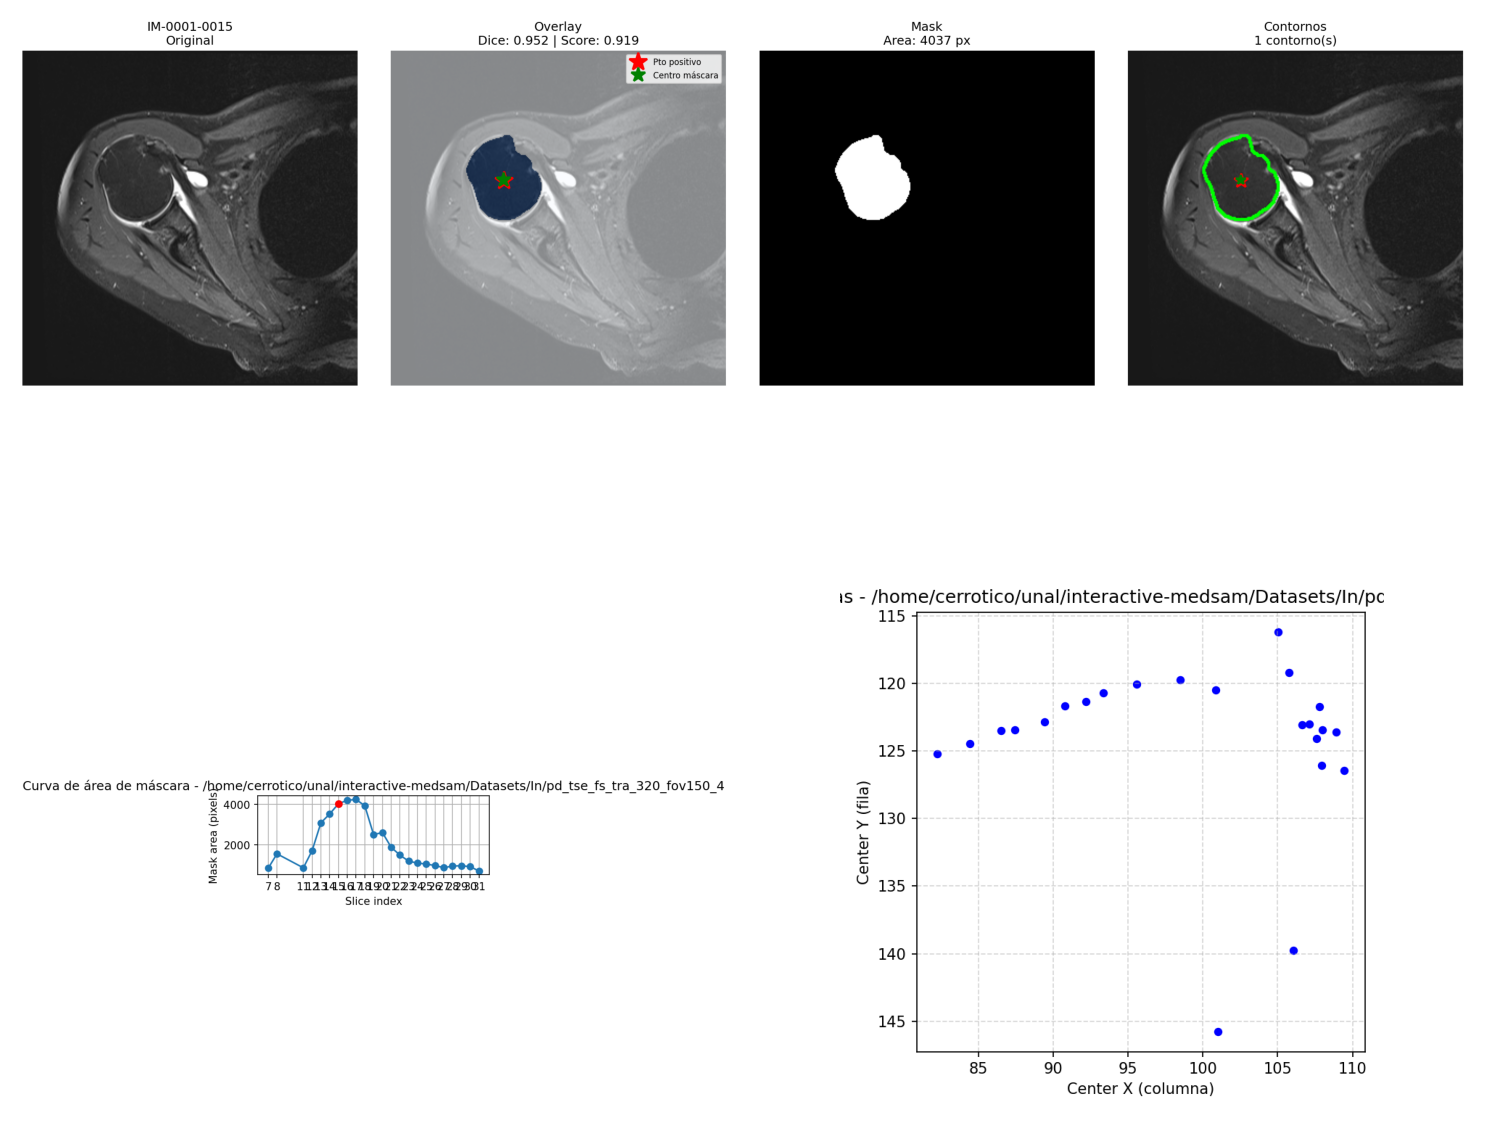
\includegraphics[width=\linewidth]{figures/seg_example.png}
      \\[0.2em]
      {\footnotesize Axial PD-fs slice with humeral segmentation overlay\\ \textit{(PixelSpacing $\approx$ 0.47\,mm; matrix 320$\times$320)}}
    \end{column}
  \end{columns}
\end{frame}

% Slide 4 -- Anatomy to geometry
\begin{frame}{From anatomy to geometry: two natural primitives}
  \begin{columns}[T]
    \begin{column}{0.5\textwidth}
      \begin{block}{The humeral head $\approx$ spherical cap}
        \begin{itemize}
          \item Articular cartilage covers a near-perfect spherical surface (radius $\sim$23--26\,mm in adults).
          \item Motivates a \alert{global sphere fit} as a patient-specific anatomical reference.
        \end{itemize}
      \end{block}
      \begin{block}{The articular surface $\approx$ local circles}
        \begin{itemize}
          \item In equatorial axial slices, the contact contour with the glenoid is locally circular.
          \item Motivates \alert{per-slice circles} that \emph{lie on} the articular surface (not approximate it).
        \end{itemize}
      \end{block}
      \begin{block}{Anatomical asymmetry}
        \begin{itemize}
          \item \textbf{Head}: closes \alert{abruptly} at the anatomical neck.
          \item \textbf{Shaft}: tapers \alert{gradually} (longer, smoother).
        \end{itemize}
      \end{block}
    \end{column}
    \begin{column}{0.5\textwidth}
      \centering
      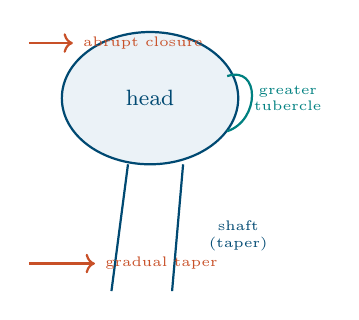
\begin{tikzpicture}[scale=0.7]
        % Sagittal sketch of proximal humerus
        \draw[thick, medBlue, fill=medSoft]
          (0,0) ellipse (1.6 and 1.2);
        \node[medBlue] at (0,0) {\footnotesize head};
        % Tubercles
        \draw[thick, medTeal] (1.4,0.4) .. controls (2.0,0.6) and (2.0,-0.4) .. (1.4,-0.6);
        \node[medTeal, font=\tiny, align=center] at (2.5,0) {greater\\tubercle};
        % Shaft
        \draw[thick, medBlue] (-0.4,-1.2) -- (-0.7,-3.5);
        \draw[thick, medBlue] (0.6,-1.2) -- (0.4,-3.5);
        \node[medBlue, font=\tiny, align=center] at (1.6,-2.5) {shaft\\(taper)};
        % Curve hint
        \draw[->, thick, medAccent] (-2.2,1.0) -- (-1.4,1.0)
          node[right, font=\tiny] {abrupt closure};
        \draw[->, thick, medAccent] (-2.2,-3.0) -- (-1.0,-3.0)
          node[right, font=\tiny] {gradual taper};
      \end{tikzpicture}
      \\[0.4em]
      {\footnotesize Anatomy directly motivates two thresholds in the pipeline:\\ \textbf{30\%} on the head side, \textbf{10\%} on the shaft side.}
    \end{column}
  \end{columns}
\end{frame}

% Slide 5 -- Hypothesis & objective
\begin{frame}{Hypothesis and objective}
  \begin{block}{Hypothesis}
    A rotator cuff tear produces a \alert{focal, geometrically detectable} discontinuity of the humeral
    articular contour. If we extract clinically interpretable geometric features from MRI, we can
    \alert{localize} the lesion to a specific tendon insertion sector --- without training a new neural network.
  \end{block}

  \begin{block}{Objective}
    Build an \alert{end-to-end pipeline} that:
    \begin{enumerate}
      \item Segments the humerus across the entire axial volume from a \alert{single seed slice}.
      \item Extracts two interpretable features:
        \textbf{(1)} \alert{circular arcs} on individual slices to identify those that lie on the articular surface;
        \textbf{(2)} the approximating \alert{sphere} that contains the articular surface.
      \item Uses these two mathematical objects to place the tear in the muscular complex of the rotator cuff.
    \end{enumerate}
  \end{block}
\end{frame}

% Slide 5b -- Design principles
\begin{frame}{Design principles}
  \begin{block}{Interpretable}
    Every output is geometrically meaningful and \alert{visually verifiable} by a radiologist:
    masks, boundary CSVs, fitted circles, summary figures.
  \end{block}

  \begin{block}{Vendor-agnostic}
    Works on SIEMENS, GE and Philips data \alert{without retraining}: thresholds are geometric (mm, \% of peak), not intensity-based.
  \end{block}

  \begin{block}{Anatomy-aware}
    Pipeline parameters reflect humeral anatomy (head vs shaft asymmetry, articular surface localization), \alert{not arbitrary heuristics}.
  \end{block}
\end{frame}

% Slide 6 -- Pipeline overview
\begin{frame}{Pipeline overview}
  \begin{center}
  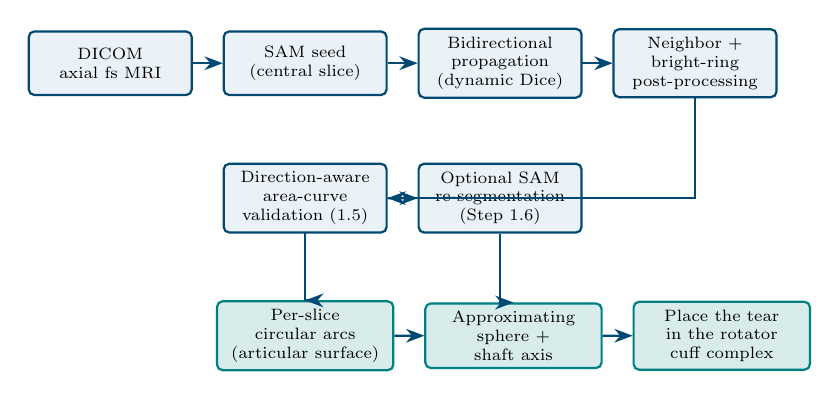
\begin{tikzpicture}[
    scale=0.85, transform shape,
    node distance=0.4cm and 0.45cm,
    box/.style={
      rectangle, rounded corners=2pt, draw=medBlue, thick, fill=medSoft,
      text width=2.2cm, align=center, minimum height=0.95cm, font=\scriptsize
    },
    feat/.style={
      rectangle, rounded corners=2pt, draw=medTeal, thick, fill=medTeal!15,
      text width=2.4cm, align=center, minimum height=0.95cm, font=\scriptsize
    },
    arr/.style={->, thick, medBlue, >=Stealth}
  ]
    \node[box] (dicom) {DICOM\\axial fs MRI};
    \node[box, right=of dicom] (sam) {SAM seed\\(central slice)};
    \node[box, right=of sam] (prop) {Bidirectional\\propagation\\(dynamic Dice)};
    \node[box, right=of prop] (post) {Neighbor +\\bright-ring\\post-processing};

    \node[box, below=1.0cm of sam] (val) {Direction-aware\\area-curve\\validation (1.5)};
    \node[box, right=of val] (resam) {Optional SAM\\re-segmentation\\(Step 1.6)};

    \node[feat, below=1.0cm of val] (circles) {Per-slice\\circular arcs\\(articular surface)};
    \node[feat, right=of circles] (sphere) {Approximating\\sphere +\\shaft axis};
    \node[feat, right=of sphere] (locate) {Place the tear\\in the rotator\\cuff complex};

    \draw[arr] (dicom) -- (sam);
    \draw[arr] (sam) -- (prop);
    \draw[arr] (prop) -- (post);
    \draw[arr] (post.south) |- (val.east);
    \draw[arr] (val) -- (resam);
    \draw[arr] (val.south) |- (circles.north);
    \draw[arr] (resam.south) |- (sphere.north);
    \draw[arr] (circles) -- (sphere);
    \draw[arr] (sphere) -- (locate);
  \end{tikzpicture}
  \end{center}

  \vspace{0.4em}
  {\footnotesize \textcolor{medTeal}{Foundation model (SAM, frozen) + classical geometry + clinical anatomy.}\\
  Each block produces auditable artifacts: masks, CSVs, validation reports, summary figures.}
\end{frame}

% Slide 7 -- SAM segmentation + propagation
\begin{frame}{Stage 1: SAM segmentation + bidirectional propagation}
  \begin{columns}[T]
    \begin{column}{0.55\textwidth}
      \begin{block}{Foundation-model segmentation}
        \footnotesize
        \begin{itemize}
          \item \alert{SAM (ViT-B)} as a frozen segmenter --- no training, no labels.
          \item One seed slice (click \emph{or} automatic point at $0.40 W, 0.40 H$).
          \item Morphological refinement: small-object removal, hole filling, opening/closing.
        \end{itemize}
      \end{block}

      \begin{block}{Bidirectional propagation, dynamic Dice}
        \footnotesize Centroid of slice $i$ $\to$ positive prompt for $i\!\pm\!1$. \alert{Adaptive threshold}:
        \[
          \tau_i = 0.45 + 0.25 \cdot |i - i_\text{seed}| / \Delta_\text{max}
        \]
        Strict near the seed, permissive at extremes. \alert{Negative-prompt} fallback for failures.
      \end{block}
    \end{column}
    \begin{column}{0.45\textwidth}
      \centering
      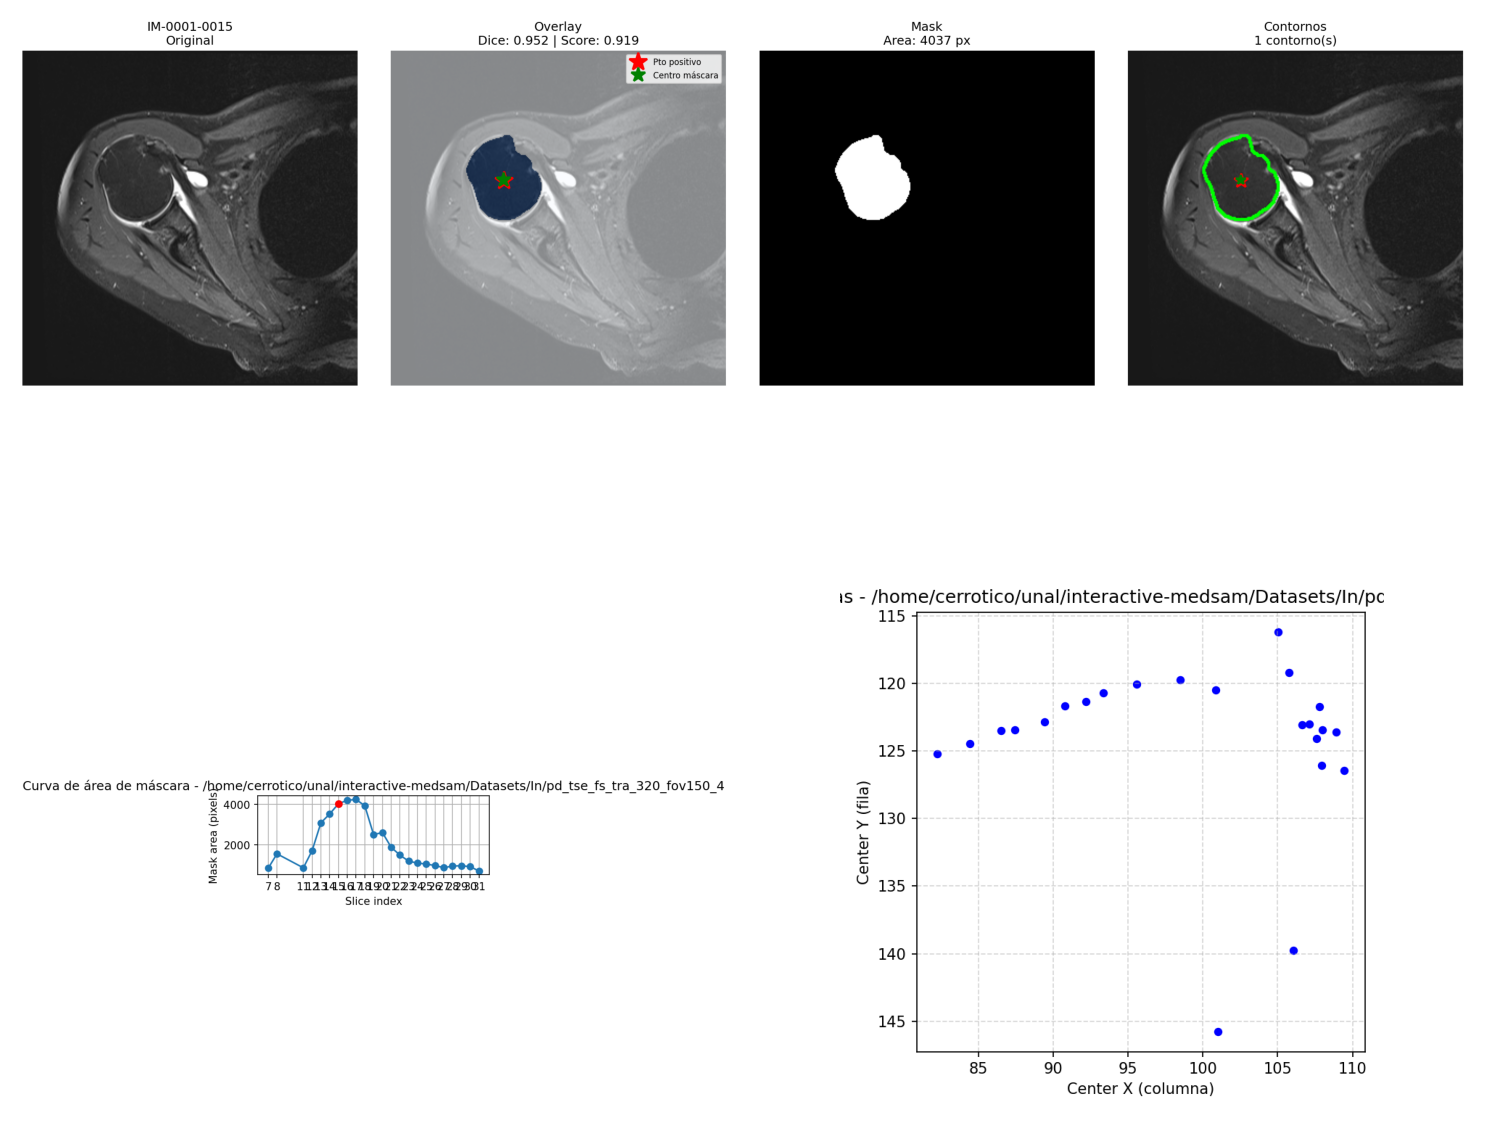
\includegraphics[width=\linewidth]{figures/seg_example.png}
      \\[0.3em]
      {\footnotesize Per-slice segmentation overlay.\\ Green = mask boundary;\\ red dot = positive prompt centroid.}
    \end{column}
  \end{columns}
\end{frame}

% Slide 8 -- Direction-aware area-curve validation (consolidated)
\begin{frame}{Stage 2: validating the area curve}
  \begin{columns}[T]
    \begin{column}{0.5\textwidth}
      \begin{block}{Read direction from the DICOM header}
        We compute the slice normal from \texttt{ImageOrientationPatient} to detect \alert{which end of the volume is the head}, instead of trusting vendor conventions.
      \end{block}
      \begin{block}{Two jobs}
        \begin{itemize}
          \item \alert{Trim} non-humeral tails (anatomy-driven thresholds).
          \item \alert{Flag} internal outliers (slices where SAM grabbed extra tissue).
        \end{itemize}
      \end{block}
    \end{column}
    \begin{column}{0.5\textwidth}
      \centering
      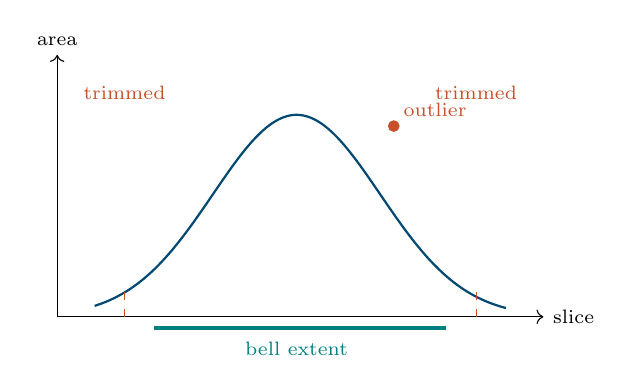
\begin{tikzpicture}[scale=0.95]
        \draw[->] (0,0) -- (6.5,0) node[right, font=\scriptsize] {slice};
        \draw[->] (0,0) -- (0,3.5) node[above, font=\scriptsize] {area};
        \draw[thick, medBlue, smooth, samples=80, domain=0.5:6.0]
          plot (\x, {2.7*exp(-pow(\x-3.2,2)/2.5)});
        \draw[medAccent, dashed] (0.9,0) -- (0.9,0.4);
        \draw[medAccent, dashed] (5.6,0) -- (5.6,0.4);
        \node[font=\scriptsize, medAccent] at (0.9,3.0) {trimmed};
        \node[font=\scriptsize, medAccent] at (5.6,3.0) {trimmed};
        \filldraw[medAccent] (4.5,2.55) circle (2pt);
        \node[medAccent, font=\scriptsize, above right] at (4.5,2.55) {outlier};
        \draw[medTeal, very thick] (1.3,-0.15) -- (5.2,-0.15);
        \node[medTeal, font=\scriptsize, below] at (3.2,-0.2) {bell extent};
      \end{tikzpicture}
      \\[0.3em]
      {\scriptsize Trim tails and flag anomalies \emph{before} fitting any geometry.}
    \end{column}
  \end{columns}
\end{frame}

% Slide 9 -- Feature 1: global sphere (consolidated)
\begin{frame}{Feature 1: global humeral-head sphere}
  \begin{columns}[T]
    \begin{column}{0.55\textwidth}
      \begin{block}{What it is}
        A single sphere fitted, in \alert{millimeters}, to the 3D points on the articular surface.
      \end{block}
      \begin{block}{How}
        \begin{itemize}
          \item \alert{K{\aa}sa} algebraic fit --- fast, linear, exact in closed form.
          \item Wrapped in \alert{RANSAC} (2000 iterations, 2 mm inlier distance) to ignore outliers like the shaft or tubercles.
        \end{itemize}
      \end{block}
      \begin{block}{Why it matters}
        Provides a patient-specific \alert{reference geometry} against which local deviations stand out.
      \end{block}
    \end{column}
    \begin{column}{0.45\textwidth}
      \centering
      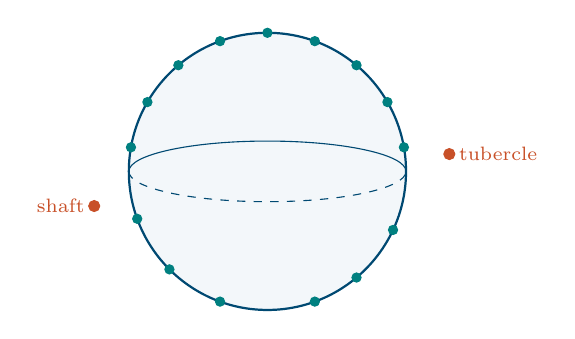
\begin{tikzpicture}[scale=1.1]
        \draw[thick, medBlue, fill=medSoft, fill opacity=0.6] (0,0) circle (1.6);
        \draw[medBlue, dashed] (-1.6,0) arc (180:360:1.6 and 0.35);
        \draw[medBlue] (-1.6,0) arc (180:0:1.6 and 0.35);
        \foreach \a in {10,30,...,170}{
          \filldraw[medTeal] ({1.6*cos(\a)},{1.6*sin(\a)}) circle (1.5pt);
        }
        \foreach \a in {200,225,250,290,310,335}{
          \filldraw[medTeal] ({1.6*cos(\a)},{1.6*sin(\a)}) circle (1.5pt);
        }
        \filldraw[medAccent] (2.1,0.2) circle (1.8pt);
        \filldraw[medAccent] (-2.0,-0.4) circle (1.8pt);
        \node[medAccent, font=\scriptsize, right] at (2.1,0.2) {tubercle};
        \node[medAccent, font=\scriptsize, left] at (-2.0,-0.4) {shaft};
      \end{tikzpicture}
      \\[0.3em]
      {\scriptsize Teal: inliers. Orange: outliers, excluded automatically.}
    \end{column}
  \end{columns}
\end{frame}

% Slide 10 -- Feature 2: per-slice circles (consolidated)
\begin{frame}{Feature 2: per-slice articular circles}
  \begin{columns}[T]
    \begin{column}{0.5\textwidth}
      \begin{block}{Key idea}
        On equatorial slices, the articular contour is locally circular. Each fitted circle is an \alert{arc that lies on the cartilage} --- not an approximation of it.
      \end{block}
      \begin{block}{Clinical meaning}
        \begin{itemize}
          \item A focal \alert{drop in inlier ratio} signals loss of articular continuity --- a potential tear.
          \item Each circle is rendered as a PNG so the radiologist can \alert{verify it slice by slice}.
        \end{itemize}
      \end{block}
    \end{column}
    \begin{column}{0.5\textwidth}
      \centering
      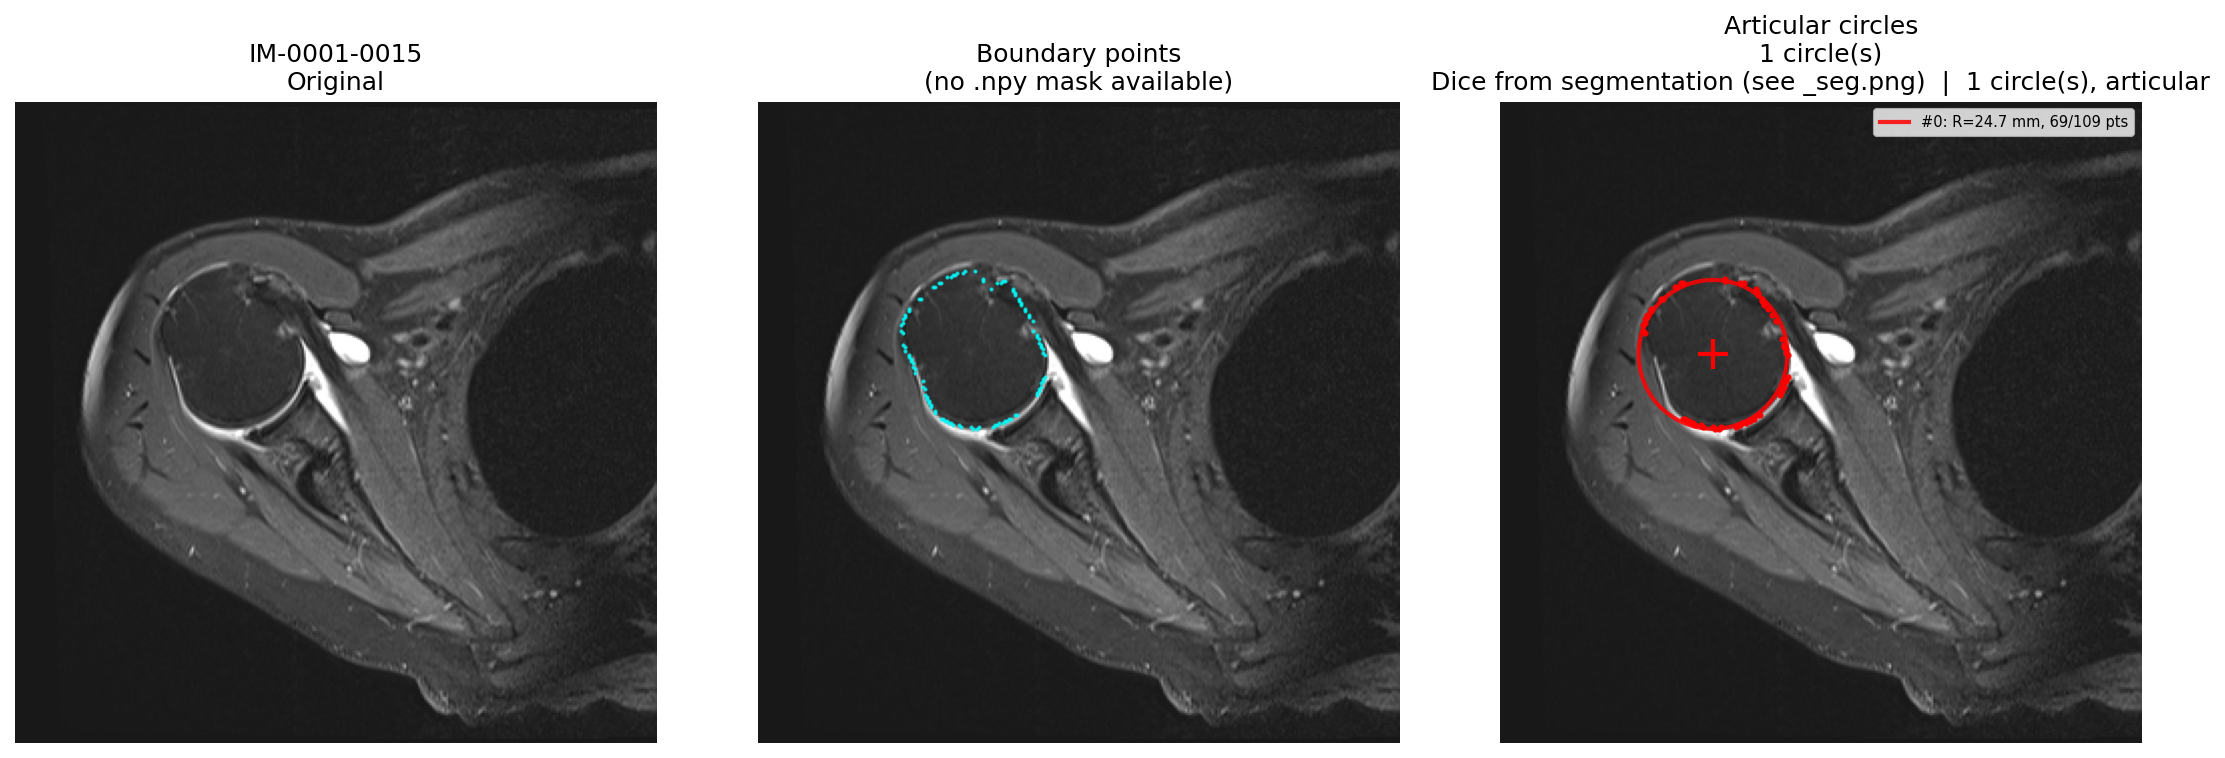
\includegraphics[width=\linewidth,height=0.7\textheight,keepaspectratio]{figures/circle_articular.png}
      \\[0.3em]
      {\scriptsize Image $\rightarrow$ mask $\rightarrow$ contour $\rightarrow$ fitted circle.}
    \end{column}
  \end{columns}
\end{frame}

% Slide 11 -- The geometric trick: parameterizing the circle
\begin{frame}{The geometric trick: parameterizing the articular circle}
  \begin{columns}[T]
    \begin{column}{0.55\textwidth}
      \begin{block}{From a circle to a 1D angular map}
        Each per-slice circle has an in-plane basis $(\mathbf{u},\mathbf{v})$ and center $\mathbf{c}$.
        Any inlier $\mathbf{p}$ has angular coordinate
        \[
          \theta = \mathrm{atan2}\big((\mathbf{p}-\mathbf{c})\!\cdot\!\mathbf{v},\; (\mathbf{p}-\mathbf{c})\!\cdot\!\mathbf{u}\big).
        \]
      \end{block}

      \begin{block}{Why this is powerful}
        The articular circle becomes a \alert{1D tendon map}:
        each $\theta$ on the circle corresponds to a known anatomical direction at the humeral head.
      \end{block}
    \end{column}
    \begin{column}{0.45\textwidth}
      \centering
      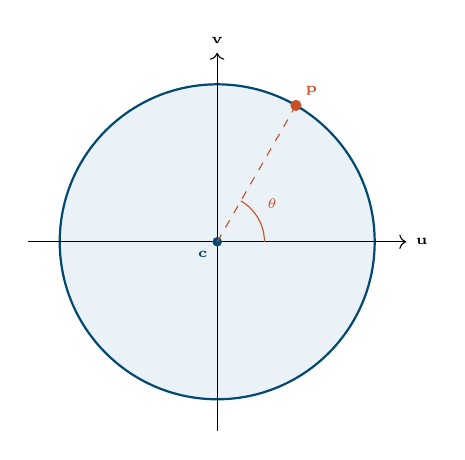
\begin{tikzpicture}[scale=1.0]
        \filldraw[medSoft] (0,0) circle (2.0);
        \draw[thick, medBlue] (0,0) circle (2.0);
        \draw[->] (-2.4,0) -- (2.4,0) node[right, font=\tiny] {$\mathbf{u}$};
        \draw[->] (0,-2.4) -- (0,2.4) node[above, font=\tiny] {$\mathbf{v}$};
        \filldraw[medBlue] (0,0) circle (1.5pt);
        \node[medBlue, font=\tiny, below left] at (0,0) {$\mathbf{c}$};
        \filldraw[medAccent] (60:2.0) circle (1.8pt);
        \draw[medAccent, dashed] (0,0) -- (60:2.0);
        \node[medAccent, font=\tiny, above right] at (60:2.0) {$\mathbf{p}$};
        \draw[medAccent] (0.6,0) arc (0:60:0.6);
        \node[medAccent, font=\tiny] at (35:0.85) {$\theta$};
      \end{tikzpicture}
    \end{column}
  \end{columns}
\end{frame}

% Slide 11b -- Anatomical sector mapping
\begin{frame}{Angular sectors $\to$ rotator-cuff tendons}
  \begin{columns}[T]
    \begin{column}{0.5\textwidth}
      \begin{block}{Anatomical sector mapping}
        Tendon insertions fall in \alert{predictable sectors}:
        \begin{itemize}
          \item \textbf{Subscapularis}: $\sim 0$--$45^\circ$.
          \item \textbf{Supraspinatus}: $\sim 45$--$135^\circ$.
          \item \textbf{Infraspinatus}: $\sim 135$--$225^\circ$.
          \item \textbf{Teres minor}: $\sim 225$--$270^\circ$.
        \end{itemize}
      \end{block}

      \begin{block}{Localization rule}
        A focal drop in inlier ratio in a sector $\to$ \alert{candidate tear} in the corresponding tendon, at the slice where the drop occurs.
      \end{block}
    \end{column}
    \begin{column}{0.5\textwidth}
      \centering
      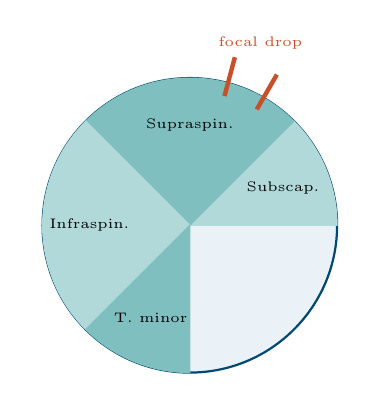
\begin{tikzpicture}[scale=0.85]
        \filldraw[medSoft] (0,0) circle (2.2);
        \draw[thick, medBlue] (0,0) circle (2.2);
        \filldraw[medTeal!30] (0,0) -- (2.2,0) arc (0:45:2.2) -- cycle;
        \filldraw[medTeal!50] (0,0) -- (45:2.2) arc (45:135:2.2) -- cycle;
        \filldraw[medTeal!30] (0,0) -- (135:2.2) arc (135:225:2.2) -- cycle;
        \filldraw[medTeal!50] (0,0) -- (225:2.2) arc (225:270:2.2) -- cycle;
        \node[font=\tiny] at (22:1.5) {Subscap.};
        \node[font=\tiny] at (90:1.5) {Supraspin.};
        \node[font=\tiny] at (180:1.5) {Infraspin.};
        \node[font=\tiny] at (247:1.5) {T. minor};
        \draw[medAccent, ultra thick] (60:2.0) -- (60:2.6);
        \draw[medAccent, ultra thick] (75:2.6) -- (75:2.0);
        \node[medAccent, font=\tiny, above] at (67:2.7) {focal drop};
      \end{tikzpicture}
      \\[0.3em]
      {\footnotesize The articular circle becomes a 1D \emph{tendon map}.}
    \end{column}
  \end{columns}
\end{frame}

% Slide 12 -- Multi-vendor robustness
\begin{frame}{Multi-vendor robustness and equity of access}
  \begin{columns}[T]
    \begin{column}{0.45\textwidth}
      \begin{block}{Tested across vendors and sites}
        \footnotesize
        \begin{itemize}
          \item \textbf{SIEMENS} -- Quibd\'o, PD-fs TSE.
          \item \textbf{GE} -- Optima MR360, Bogot\'a, PD-fs FSE.
          \item \textbf{Philips} -- Ingenia, SOMA, ePDW SPAIR.
          \item Matrix 256$\times$256 to 320$\times$320; PD-fs and T1-fs.
        \end{itemize}
      \end{block}

      \begin{block}{Why this generalizes}
        \footnotesize
        \begin{itemize}
          \item Frozen SAM $\Rightarrow$ no domain-specific weights to overfit.
          \item Thresholds are \alert{geometric} (mm, \% of peak), not intensity-based.
          \item Direction handling reads DICOM headers, not vendor conventions.
        \end{itemize}
      \end{block}
    \end{column}
    \begin{column}{0.55\textwidth}
      \footnotesize
      \begin{tabular}{@{}lcc@{}}
        \toprule
        \textbf{Dataset} & \textbf{Kept} & \textbf{Articular} \\
        \midrule
        SIEMENS P5SE1 (Quibdó)        & 21/32 & 5 \\
        SIEMENS PD fs (fov150)        & 18/23 & 4 \\
        SIEMENS T1 fs \#5             & 19/24 & 5 \\
        SIEMENS T1 fs \#11            & 17/22 & 4 \\
        GE Optima MR360 (Bogotá)      & 16/21 & 4 \\
        Philips Ingenia (SOMA)        & 20/26 & 5 \\
        \bottomrule
      \end{tabular}
      \vspace{0.4em}

      \begin{block}{Equity-of-access angle}
        \footnotesize Datasets include \alert{Quibd\'o, Choc\'o}, a region with limited subspecialty radiology. Vendor-agnostic, interpretable AI directly supports diagnostic capacity in such settings.
      \end{block}
    \end{column}
  \end{columns}
\end{frame}

% Slide 13 -- Qualitative results: full-figure
\begin{frame}{Qualitative results: per-dataset summary}
  \centering
  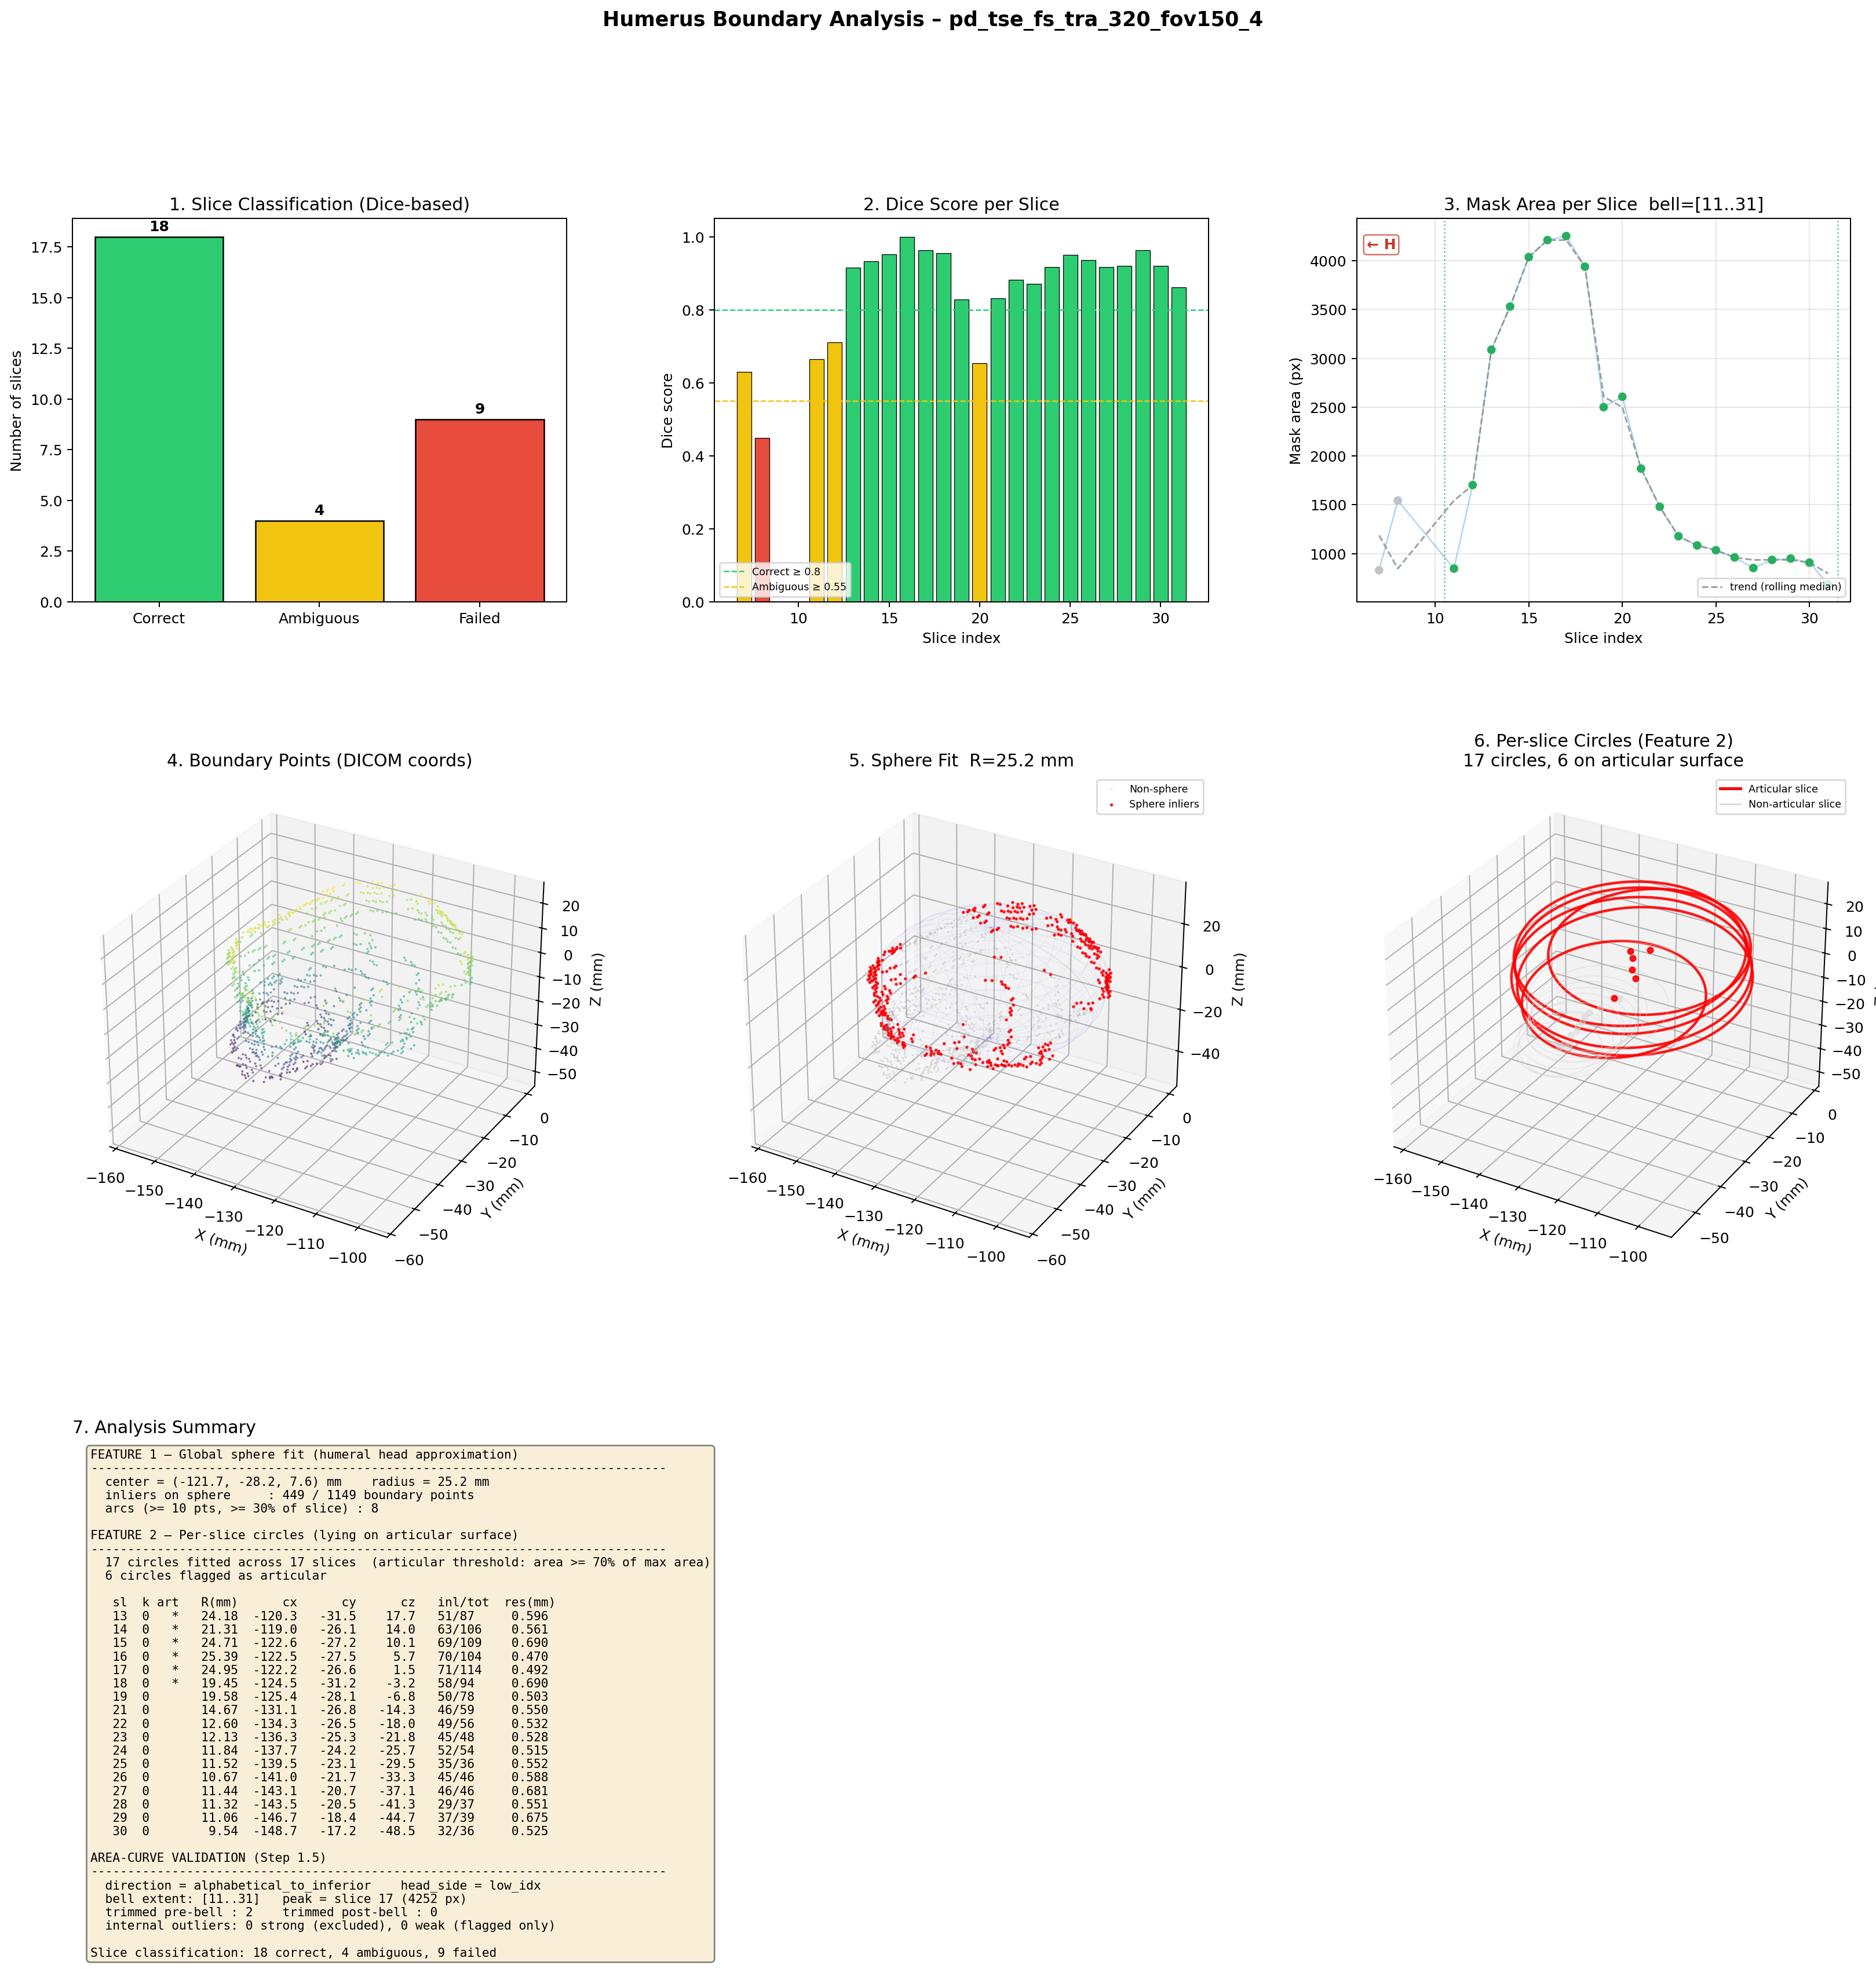
\includegraphics[height=0.75\textheight,keepaspectratio]{figures/summary_pd4.png}
  \\[0.3em]
  {\footnotesize Summary for dataset \textit{pd\_tse\_fs\_tra\_320\_fov150\_4}: mask boundaries,
  area curve with Step 1.5 status, slice-circle centers and reconstructed surface.}
\end{frame}

% Slide 13b -- How to read the figure
\begin{frame}{How to read the summary figure}
  \begin{columns}[T]
    \begin{column}{0.55\textwidth}
      \begin{block}{Color code (panel 3, area curve)}
        \begin{itemize}
          \item \textcolor{green!50!black}{\textbf{Green}}: slices kept for analysis.
          \item \textcolor{gray}{\textbf{Gray}}: tails trimmed by direction-aware logic.
          \item \textcolor{red}{\textbf{Red}}: strong outliers excluded after Pass 2.
          \item Vertical lines: bell-extent boundaries.
          \item Caret \texttt{H$\rightarrow$}: which side of the volume is the head.
        \end{itemize}
      \end{block}
    \end{column}
    \begin{column}{0.45\textwidth}
      \begin{block}{Auditability by design}
        Every slice exports a five-panel \texttt{*\_circle.png} (image, mask, contour, fitted circle, overlay). A radiologist can verify each fit \alert{slice by slice}, not just trust an aggregate score.
      \end{block}

      \begin{block}{Reproducibility}
        All thresholds are exposed as CLI flags;
        every run writes \texttt{area\_curve\_validation.csv} for downstream audit.
      \end{block}
    \end{column}
  \end{columns}
\end{frame}

% Slide 14 -- Limitations & clinical considerations
\begin{frame}{Limitations and clinical considerations}
  \begin{columns}[T]
    \begin{column}{0.5\textwidth}
      \begin{block}{Current limitations}
        \begin{itemize}\small
          \item \textbf{Validation cohort size}: 6 datasets across 3 vendors --- proof of concept, not clinical validation.
          \item \textbf{Seed-slice selection}: automatic point at $(0.40W, 0.40H)$ assumes typical centering; pathological positioning may fail.
          \item \textbf{Pattern B without GPU}: when SAM grabs adjacent muscle/glenoid, weak outliers are flagged but not re-segmented unless GPU + SAM are available (Step 1.6).
          \item \textbf{Tear-localization rule is a hypothesis}: the angular-sector mapping needs prospective validation against arthroscopic ground truth.
        \end{itemize}
      \end{block}
    \end{column}
    \begin{column}{0.5\textwidth}
      \begin{block}{What is required for clinical translation}
        \begin{itemize}\small
          \item \alert{Multi-center, larger cohort} with arthroscopy or surgical confirmation.
          \item Inter-reader study: do radiologists agree with the geometric flag location?
          \item Integration with PACS / DICOM-SR for routine workflow.
          \item Reproducibility: containerized pipeline, public benchmarks.
        \end{itemize}
      \end{block}

      \begin{block}{Risk profile}
        Because outputs are \alert{geometric, visualized, and auditable}, the system fails ``loudly''
        rather than silently --- a key property for clinical deployment compared to opaque end-to-end models.
      \end{block}
    \end{column}
  \end{columns}
\end{frame}

% Slide 15 -- Conclusion
\begin{frame}{Conclusions and next steps}
  \begin{block}{Take-home messages}
    \footnotesize
    \begin{itemize}
      \item A \alert{frozen foundation model} (SAM) plus \alert{anatomy-aware classical geometry} produces interpretable shoulder MRI features without training.
      \item DICOM-header reading makes the pipeline \alert{direction-aware} with asymmetric anatomy-driven thresholds.
      \item Two features (humeral sphere + per-slice articular circles) enable \alert{tear localization by angular sector}.
      \item Robust across SIEMENS, GE, Philips; relevant for low-resource radiology settings.
    \end{itemize}
  \end{block}

  \begin{columns}[T]
    \begin{column}{0.5\textwidth}
      \begin{block}{Next steps}
        \begin{itemize}\footnotesize
          \item Implement the angular-sector $\to$ tendon mapping end-to-end.
          \item Prospective validation against arthroscopy.
          \item Inter-reader and inter-vendor reproducibility study.
          \item Integration into a clinical reading viewer.
        \end{itemize}
      \end{block}
    \end{column}
    \begin{column}{0.5\textwidth}
      \begin{block}{Acknowledgements}
        \begin{itemize}\footnotesize
          \item Universidad Nacional de Colombia --- Topics in Computational Geometry.
          \item Clínica Especialistas Reina Virgen María (Quibdó), Clínica Santa Ana (Bogotá), SOMA Radiology.
          \item Open-source: SAM (Meta AI), pydicom, scikit-image, OpenCV, NumPy/SciPy.
        \end{itemize}
      \end{block}
    \end{column}
  \end{columns}

  \vspace{0.4em}
  \begin{center}
    \large \textcolor{medBlue}{\textbf{Thank you --- questions welcome.}}\\
    \footnotesize \textit{1\textsuperscript{st} UEMS Congress 2026 --- Leuven, Belgium}
  \end{center}
\end{frame}


\end{document}
